\documentclass[parskip=full]{scrartcl}
\usepackage[top=2.54cm, bottom=2.54cm, left=2.54cm, right=2.54cm]{geometry}
\usepackage[utf8]{inputenc} % use utf8 file encoding for TeX sources
\usepackage[T1]{fontenc}    % avoid garbled Unicode text in pdf
\usepackage[ngerman]{babel}  % german hyphenation, quotes, etc
\usepackage{hyperref}
\usepackage{enumerate}
\usepackage[shortlabels]{enumitem}
\usepackage[dvipsnames]{xcolor}
\usepackage{graphicx}
\usepackage{mwe}
\usepackage{caption}
\usepackage{adjustbox}

% Set footer and header bar
\usepackage[headsepline, footsepline]{scrlayer-scrpage}
\addtokomafont{headsepline}{\color{BlueViolet}}
\addtokomafont{footsepline}{\color{BlueViolet}}
\KOMAoptions{headsepline=1.25pt:\textwidth}
\KOMAoptions{footsepline=1.25pt:\textwidth}
\clearpairofpagestyles
\rofoot{\thepage}
\ihead{Write your own Android App: Recishare}

\hypersetup{
    pdftitle={PSE: Pflichtenheft},
    colorlinks,
    linkcolor={black!50!black},
    citecolor={blue!50!black},
    urlcolor={blue!80!black}
}
\usepackage{csquotes}
% detailed hyperlink/pdf configuration
% ‘texdoc hyperref‘ for options
% provides \enquote{} macro for "quotes"


\begin{document}
\begin{titlepage}
    \begin{center}
        \begin{Huge}
            {\textbf{Write your own Android App: Recishare}}
        \end{Huge}
        \vspace{12px}

        Praxis der Softwareentwicklung (PSE)\\
        Sommersemester 2023\\
        \vspace{150px}

        \begin{Huge}
            {\textbf{Pflichtenheft}}
        \end{Huge}
        \vspace{12px}

        Auftraggeber\\
        Karlsruher Institut für Technologie\\
        KASTEL — Institut für Informationssicherheit und Verlässlichkeit\\
        \vspace{330px}

        Auftragnehmer\\
        Karlsruher Intellektuelle\\
        Henri Becker, Konrad Knappe, Lukas Schwarz, Raphael Zipperer\\
    \end{center}
\end{titlepage}

\tableofcontents

\vspace{32px}
\section*{Gender-Hinweis}
Zur besseren Lesbarkeit wird in diesem Pflichtenheft das generische Maskulinum verwendet.
Die in diesem Heft verwendeten Personenbezeichnungen beziehen sich – sofern nicht anders kenntlich gemacht – auf alle Geschlechter.
\newpage


\section{Zielbestimmung}

\subsection{Musskriterien}
Musskriterien: unabdingbare Leistungen der Software.

\begin{enumerate}[start=1,label={$\langle$\bfseries RM\arabic*$\rangle$}, leftmargin = 5em, itemsep=4pt, parsep=4pt]
    \item Die App besitzt eine Nutzerverwaltung.
    \item Der Nutzer muss sich registrieren, einloggen und ausloggen können.
    \item Der Nutzer muss eine Gruppe erstellen und beitreten können.
    \item Der Nutzer muss Gruppen nach dem Beitreten wieder verlassen können.
    \item Es muss in jeder Gruppe mindestens ein Gruppenadmin sein.
    \item Der Nutzer muss Rezepte erstellen und hochladen können.
    \item Es müssen erstellte Rezepte von anderen Nutzern in der gleichen Gruppe angeschaut werden können.
    \item Erstellte Rezepte müssen vom Ersteller seperat verwaltet und geändert werden können.
    
   
\end{enumerate}

\subsection{Sollkriterien}
Sollkriterien: erstrebenswerte Leistungen.

\begin{enumerate}[start=1,label={$\langle$\bfseries RS\arabic*$\rangle$}, leftmargin = 5em, itemsep=4pt, parsep=4pt]
    
    \item Der Nutzer soll bei Rezepten Portionen skalieren können.
    \item Der Nutzer kann Rezepte favoritisieren.
    \item In jeder Gruppe soll es einen Gruppenadmin geben.
    \item Admins sollen Nutzer aus Gruppen entfernen können.
    \item Admins sollen Rezepte von Nutzern vor anderen Nutzern in der Gruppe ausblenden können.
    \item Zu jedem Rezept soll die Kochzeit, Schwierigkeit hinzugefügt werden können.
    \item Das Hinzufügedatum eines Rezept soll einsehbar sein.
    \item Der Nutzer soll sein Passwort wieder zurücksetzen können.
    \item Der Nutzer soll sein Konto nach erstellen wieder löschen können.
    
\end{enumerate}

\subsection{Kannkriterien}
Kannkriterien: Leistungen, die enthalten sein können.

\begin{enumerate}[start=1,label={$\langle$\bfseries RC\arabic*$\rangle$}, leftmargin = 5em, itemsep=4pt, parsep=4pt]
    \item Rezepte können in Form von PDFs exportiert werden.
    \item Man kann zwischen Dark Mode und Light Mode wechseln können.
    \item Es kann genau ein Bild zum Rezept hochladen werden.
    \item Der Nutzer soll Rezepte bewerten können. %Noch Aktuell?
    \item Der Nutzer kann Zutaten aus einer Liste auswählen.
\end{enumerate}

\subsection{Abgrenzungskriterien}
Abgrenzungskriterien: Leistungen die explizit nicht umgesetzt werden.

\begin{enumerate}[start=1,label={$\langle$\bfseries RW\arabic*$\rangle$}, leftmargin = 5em, itemsep=4pt, parsep=4pt]
    \item Es können keine Lebensmittel über die App bestellt werden.
    \item Es können keine Kommentare zu Rezepten hinzugefügt werden.
    \item Es gibt keine integrierte Chatfunktion.
    \item Es können keine Videos den Rezepten hinzugefügt werden.
    \item Es können keine Nutzer direkt über die App gesucht werden.
\end{enumerate}

\section{Produkteinsatz}
Dieses Kapitel dient dazu, den Einsatzbereich, die Zielgruppen und die Betriebsbedingungen der zu entwickelnden Software aufzuführen.

\subsection{Anwendungsbereiche}
In diesem Abschnitt wird erläutert, in welchen Bereichen die Software eingesetzt werden soll.
Die App bietet eine Reihe von Funktionen, die Nutzern eine Vielzahl an Anwendungsmöglichkeiten rund um das Thema kochen bieten. 
Zum einen können Nutzer Rezepte hochladen und diese bei Bedarf im Nachhinein bearbeiten. 
Diese Funktionen ermöglichen das Teilen von Rezepten mit anderen Nutzern. 
Zudem können sie als eine Art digitales Kochbuch benutzt werden, um eigene Rezepte zu organisieren und bei Bedarf auch von anderen Geräten aufrufen zu können. 
Außerdem können Nutzer die Rezepte anderer Nutzer betrachten, bewerten und speichern. 
Um zielgerichtet gewünschte Ergebnisse zu finden, gibt es eine Suchfunktion, mit der Nutzer Rezepte und andere Nutzer finden können. 
So können Nutzer gezielt ihre Kochkenntnisse erweitern. 
Rezepte können skaliert werden, um die richtige Menge für eine bestimmte Anzahl an Personen effizient zu ermitteln. 
Nutzer können außerdem Kochgruppen beitreten, um Rezepte mit Nutzern mit ähnlichen Interessen zu teilen. 
Die App ist explizit kein soziales Medium und besitzt dementsprechend keinerlei Chat- bzw. Kommentarsektionen.

\subsection{Zielgruppen}
Im Folgenden wird aufgezählt, für welche Anwender die Software im Wesentlichen gedacht ist. 
Die Kochapp richtet sich an alle, die gerne kochen und ihre Kocherfahrung verbessern möchten. 
Die App ist insbesondere für Gruppen geeignet, in denen gekocht wird (bsp. Wohngemeinschaften), da Rezepte effizient geteilt und skaliert werden können.

\subsection{Betriebsbedingungen}
In diesem Unterkapitel wird auf die unterschiedlichen Bedürfnisse und Anforderungen an die Software eingegangen.

\section{Produktübersicht}
In diesem Kapitel werden die Produktfunktionen beschrieben und in einem Use-Case-Diagramm visualisiert.
Das Use-Case-Diagramm zeigt mittels Verbindungslininen, wie die einzelnen Use-Cases zueinander stehen.
Der Abschnitt „Gruppenverwaltung“ und "Rezepte Liste" werden genauer in jeweils einem Aktivitätsdiagramm abgebildet.
Dadurch können die einzelnen Schritte, die durchlaufen werden, besser beschrieben werden.

\paragraph{Abbildung 3.1}
In dem Use-Case-Diagramm „Aufbau der App“ sieht man die allgemeine Struktur der App.\\
Bei der erstmaligen Nutzung muss der Nutzer sich registrieren.
Dazu muss er seinen Namen, seine E-Mail-Adresse und ein Passwort eingeben.
Das Passwort muss durch eine erneute Eingabe berstätigt werden.
Falls der Nutzer schon einen Nutzerkonto besitzt kann er sich einloggen.
Dazu muss er seine E-Mail-Adresse und sein Passwort eingeben.
Hat der Nutzer sein Passwort vergessen besteht die Möglichkeit das Passwort zurückzusetzen.
Ein eingeloggter Nutzer muss sich nicht erneut einloggen.\\
Nach dem Einloggen gelangt der Nutzer auf die Rezept-Ansicht.
Hier hat er die Möglichkeit, Rezepte zu filtern, suchen oder zu sortieren.
Durch klicken auf ein Rezept kann der Nutzer das Rezept ansehen, favorisieren und die Portionsgrößen ändern.\\
Durch klicken auf die Schaltfläche "Rezept erstellen" kann der Nutzer ein neues Rezept erstellen.
Es können Zutaten, Kochanleitung, Schwierigkeit und Kochzeit ƒür das neue Rezept angegeben werden.
Im Anschluss kann das Rezept veröffentlicht werden.\\
Durch klicken auf die Schaltfläche "Verwaltungs-Ansicht" gelangt der Nutzer auf die "Verwaltungs-Ansicht".
In dieser Ansicht kann der Nutzer sich ausloggen, sein Nutzerkonto löschen, seinen Nutzernamen ändern, 
erstellte Rezepte bearbeiten, eine Gruppe verlassen und Gruppen-Kürzel und das dazugehörige Passwort kopieren.\\
Durch das drücken der Schaltfläche "Gruppe hinzufügen" kann der Nutzer eine neue Gruppe erstellen oder beitreten.
Eine Gruppe kann durch Eingabe eines Gruppennamen und Passwort erstellt werden.\\ %Passiv
Von der Verwaltungsansicht-


\paragraph{Abbildung 3.2}
Im Aktivitätsdiagramm „Rezepte Liste“ werden die verschiedenen Möglichkeiten unter dem Menüpunkt aufgeführt.
Der Nutzer hat die Möglichkeite Rezepte durch eine Suchfeld zu suchen.
Der Nutzer hat die Möglichkeit die Rezepteliste durch vorgegebene Sortierungen zu sortieren.
Beim Auswählen eines Rezepts öffnet sich das zugehörige Rezeptfenster.
Im Rezeptfenster kann der Nutzer die Portionsgröße anpassen, das Rezept bewerten und das Rezept fovorisieren.
Im Fenster Rezeptliste kann der Nutzer Rezepte erstellen.
Es öffnet sich ein leeres Rezepttemplate Fenster.
Der Nutzer kann die Zutaten und die Kochanleitung in diesem Fenster eingeben.
Nach Bestätigung der Eingabe kommt der Nutzer wieder auf die Rezept Liste.

\paragraph{Abbildung 3.3}
Im Aktivitätsdiagramm Verwaltung  möchte der Nutzer seine Gruppen verwalten.
Es besteht die Wahl eine Gruppe zu erstellen, eine Gruppe hinzuzufügen oder bestehende Gruppen zu verwalten.
Beim erstellen einer Gruppe kann der Nutzer einen Gruppennamen und ein Passwort wählen.
Nach Bestätigung wird der Nutzer der Gruppe hinzugefügt.
Die Gruppe ist daraufhin unter Verwaltung zu finden.
Beim hinzufügen einer Gruppe muss der Nutzer das Gruppen-Kürzel und Passwort eingeben.
Bei erfolgreicher Eingabe wird der Nutzer der Gruppe hinzugefügt.
Bei fehlerhafter Eingabe erscheint eine Fehlermeldung.
Falls der Nutzer schon in einer Gruppe beigetreten ist, kann er der Gruppe austreten oder das Gruppen-Kürzel und Passwort der Gruppe kopieren.
Beim Austreten muss der Nutzer noch nachträglich bestätigen, dass er aus der austreten möchte.
\newpage

\begin{figure}[!htp]
    \centering
    \begin{adjustbox}{right=160mm}
        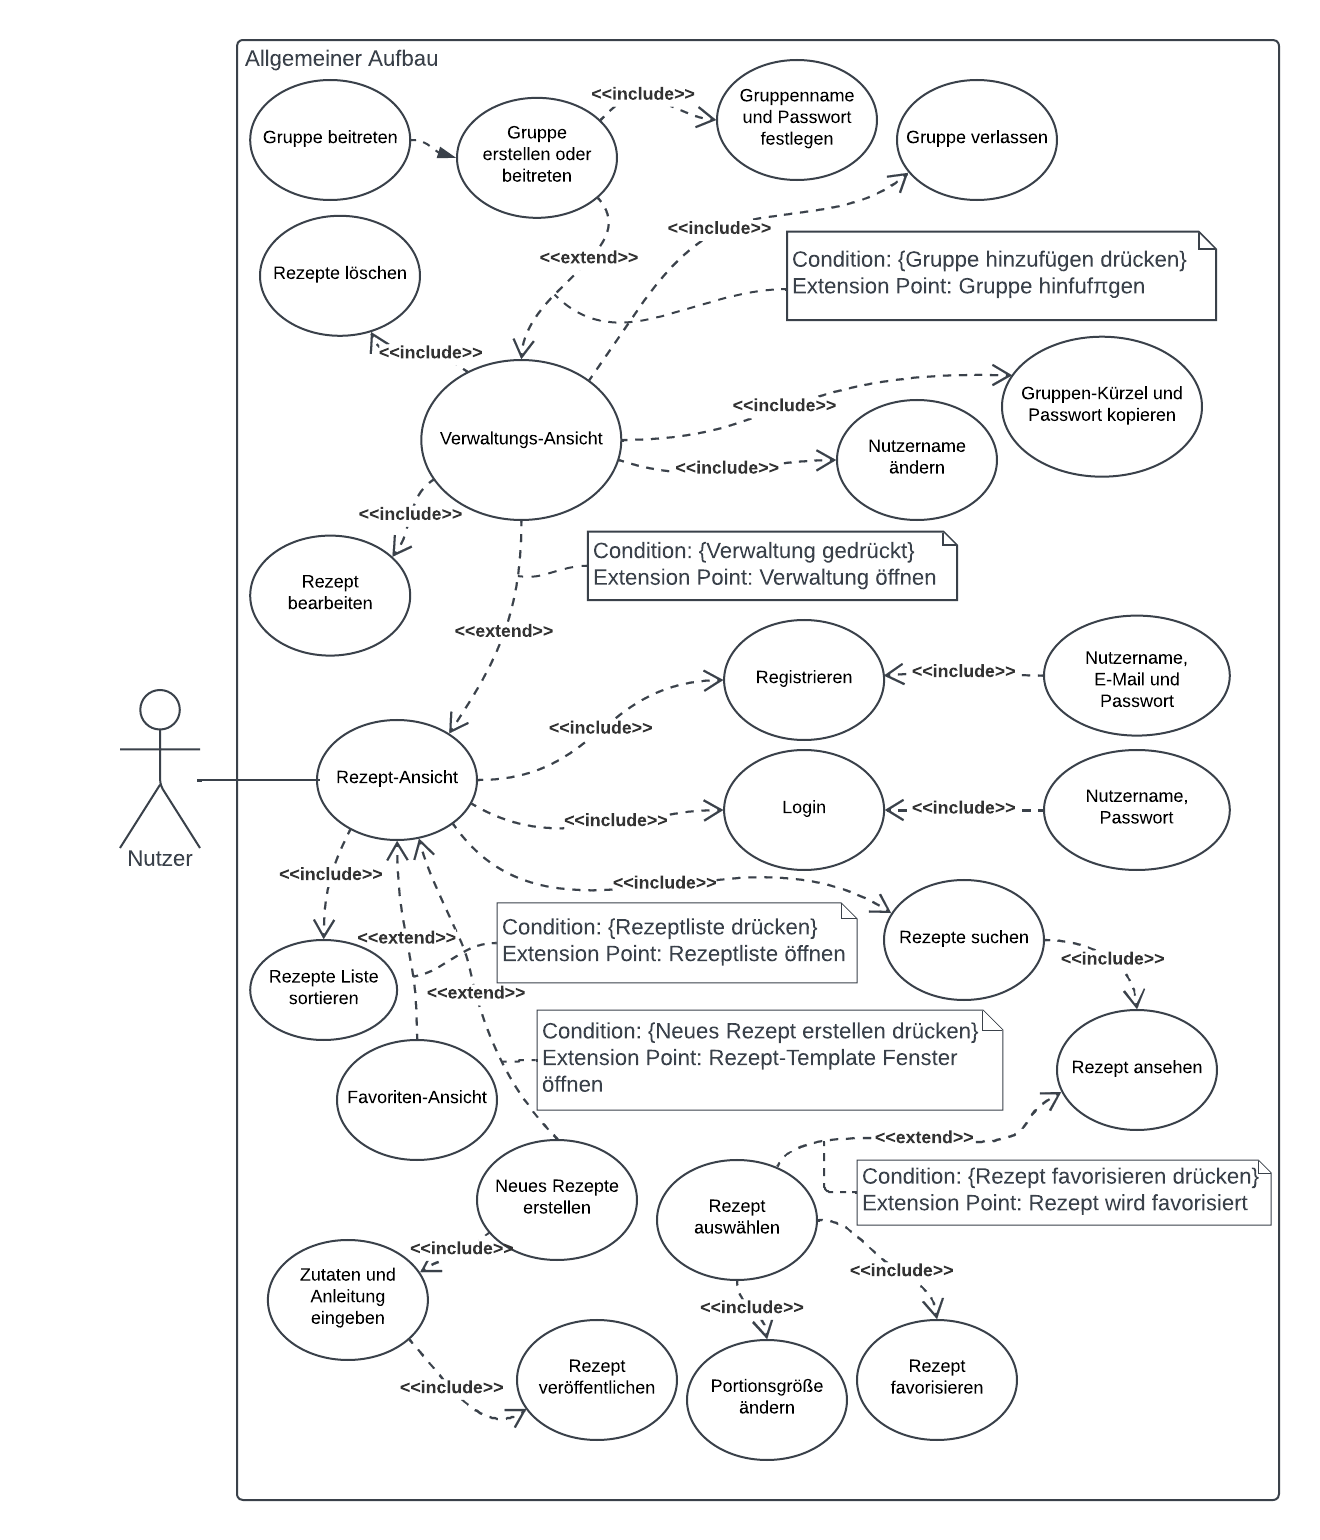
\includegraphics[height=220mm]{images/section3/Use-Case-Diagramm Aufbau App.png}
    \end{adjustbox}
    \caption*{Abbildung 3.1: Use-Case-Diagramm: Aufbau der App}
    \label{fig:A31}
\end{figure}
\newpage

\begin{figure}[!htp]
    \centering
    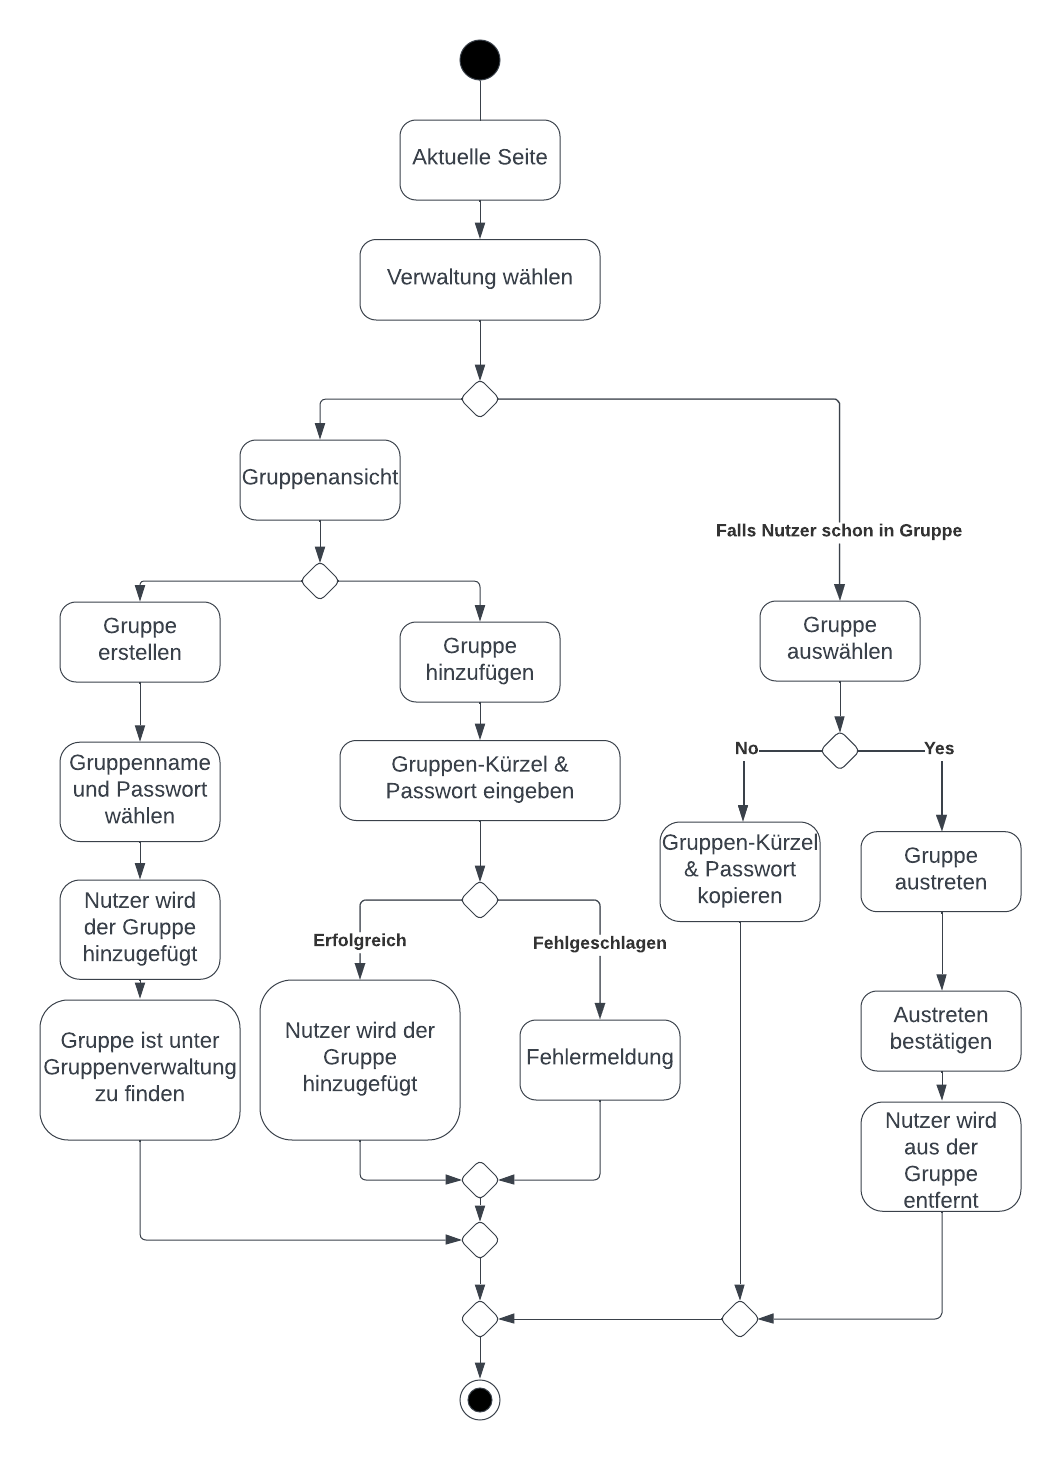
\includegraphics{images/section3/Aktivitaetsdiagramm Gruppenverwaltung.png}\\
    Abbildung 3.2: Aktivitätsdiagramm: Rezepte Liste
    \label{fig:A32}
\end{figure}
\newpage

\begin{figure}[!htp]
    \centering
    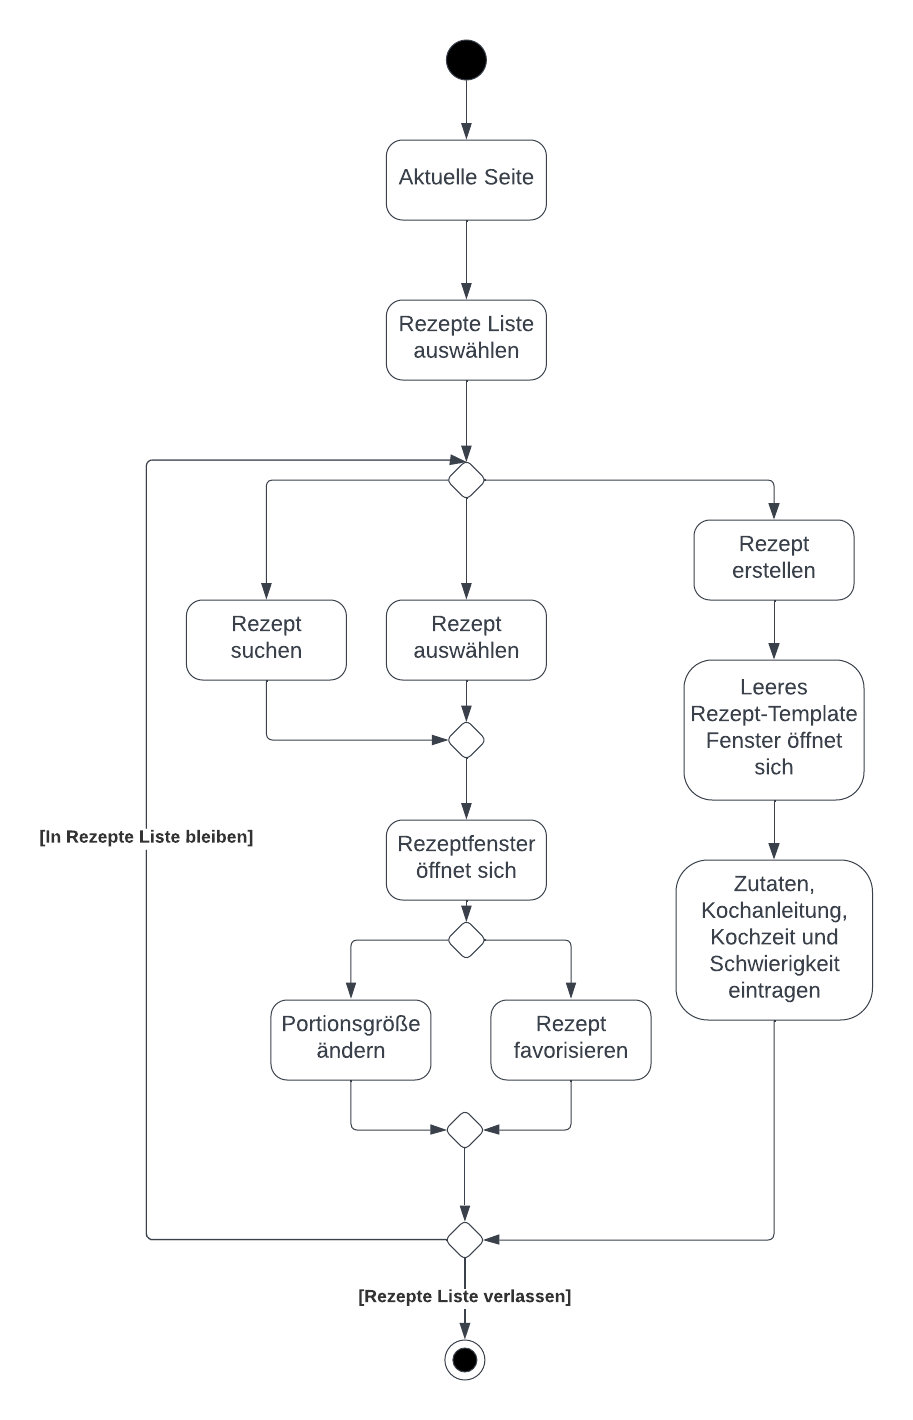
\includegraphics{images/section3/Aktivitaetsdiagramm Rezepte Liste.png}\\
    Abbildung 3.3: Aktivitätsdiagramm: Gruppenverwaltung
    \label{fig:A33}
\end{figure}
\newpage

\section{Produktfunktion}
\textbf{Einloggen $\langle$F10$\rangle$}\\
\textbf{Anwendungsfall:} Der Nutzer möchte sich in der App anmelden um alle Features der App nutzen zu können.\\
\textbf{Anforderungen:} RM1\\
\textbf{Ziel:} Der Nutzer erhält Zugang zu seinem Profil in der App indem eine Verbindung zum Server hergestellt wird.\\
\textbf{Vorbedingung:} Der Nutzer hat bereits ein Konto erstellt.\\
\textbf{Nachbedingung Erfolg:} Der Nutzer ist erfolgreich eingeloggt und wird zur Hauptansicht der App weitergeleitet.\\
\textbf{Nachbedingung Fehlschlag:} Das Passwort oder der Nutzername ist falsch, sodass ein Pop-up-Fenster erscheint mit einer Fehlermeldung.\\
\textbf{Akteure:} Nutzer, Server\\
\textbf{Auslösendes Ereignis:} Der Nutzer startet die App.\\
\textbf{Beschreibung:}
\begin{enumerate}
    \item Start der App.
    \item Login View erscheint
    \item Eingabe des Nutzernamens.
    \item Eingabe des Passworts.
    \item Auf Weiter Button klicken, um Anmeldung abzuschließen.
\end{enumerate}
\textbf{Erweiterung:} -\\
\textbf{Alternativen:} Mit einem Klick auf den Registrieren Button kann ein Nutzer Konto angelegt werden. Mit einem Klick auf den Passwort vergessen Button Knopf kann das Passwort eines bestehenden Kontos geändert werden.  \\
\newpage

\textbf{Registrierung $\langle$F20$\rangle$}\\
\textbf{Anwendungsfall:} Der Nutzer möchte ein Nutzer Konto anlegen.\\
\textbf{Anforderungen:} \\
\textbf{Ziel:} Der Nutzer legt ein Nutzerkonto an um alle Features der App nutzen zu können.\\
\textbf{Vorbedingung:} Die App muss bereits gestartet worden sein.
\textbf{Nachbedingung Erfolg:} Der Nutzer wird zum Gruppenansicht weitergeleitet und mit einem Pop-up-Fenster erfolgt die Bestätigung zur erfolgreichen Registrierung.\\
\textbf{Nachbedingung Fehlschlag:} Ein Pop-up-Fenster erscheint mit einer Fehlermeldung.\\
\textbf{Akteure:} Nutzer, Server\\
\textbf{Auslösendes Ereignis:} Der Nutzer muss auf den "Registrieren" Button in der Loginansicht klicken.\\
\textbf{Beschreibung:}
\begin{enumerate}
    \item Klick auf den Registrieren Button.
    \item Eingabe des Nutzernamens.
    \item Eingabe der E-Mail-Adresse.
    \item Eingabe eines Passworts.
    \item Wiederholen des Passworts.
    \item Klick auf den Weiter Button.
\end{enumerate}
\textbf{Erweiterung:} -\\
\textbf{Alternativen:} Durch das Klicken auf den Login Button wird der Nutzer zurück zur Loginansicht geleitet.\\
\newpage

\textbf{Passwort zurücksetzen $\langle$F20$\rangle$}\\
\textbf{Anwendungsfall:} Der Nutzer möchte das Passwort für seinen Benutzerkonto zurücksetzen.\\
\textbf{Anforderungen:} \\
\textbf{Ziel:} Der Nutzer kann eine neues Passwort setzen.\\
\textbf{Vorbedingung:} Die App muss bereits gestartet worden sein.\\
\textbf{Nachbedingung Erfolg:} Der Nutzer wird zum Loginansicht weitergeleitet und mit einem Pop-up-Fenster erfolgt die Bestätigung der Versendung einer E-Mail an die angegeben E-Mail Adresse.\\
\textbf{Nachbedingung Fehlschlag:} Ein Pop-up-Fenster erscheint mit einer Fehlermeldung.\\
\textbf{Akteure:} Nutzer, Server\\
\textbf{Auslösendes Ereignis:} Der Nutzer muss auf den Passwort vergessen Button in der Loginansicht klicken.\\
\textbf{Beschreibung:}
\begin{enumerate}
    \item Klick auf den Passwort vergessen Button.
    \item Eingabe der E-Mail Adresse.
    \item Klick auf den Weiter Button.
\end{enumerate}
\textbf{Erweiterung:} -\\
\textbf{Alternativen:} Durch das Klicken auf den Verlassen Button wird der Nutzer zurück zur Loginansicht geleitet.\\
\newpage

\textbf{Benutzernamen ändern $\langle$F30$\rangle$}\\
\textbf{Anwendungsfall:} Der Nutzer möchte seinen Benutzernamen ändern.\\
\textbf{Anforderungen:} \\
\textbf{Ziel:} Der Nutzer kann seinen Benutzernamen an seine Wünsche anpassen.\\
\textbf{Vorbedingung:} Der Nutzer muss einen Nutzerkonto haben.\\
\textbf{Nachbedingung Erfolg:} Der aktualisierte Nutzername wird anderen Nutzern angezeigt.\\
\textbf{Nachbedingung Fehlschlag:} Ein Pop-up-Fenster erscheint mit einer Fehlermeldung.\\
\textbf{Akteure:} Nutzer, Server\\
\textbf{Auslösendes Ereignis:} In der Verwaltungsansicht klickt der Nutzer auf den Nutzernamen bearbeiten Button.\\
\textbf{Beschreibung:}
\begin{enumerate}
    \item Der Nutzer klickt auf den Nutzernamen bearbeiten Button.
    \item Der neue Benutzername wird eingegeben.
    \item Der Nutzer klickt auf den speichern Button.
\end{enumerate}
\textbf{Erweiterung:} -\\
\textbf{Alternativen:} Der Nutzer kann auf den Exit Button klicken und der Prozess wird abgebrochen und der Nutzer gelangt zurück zur Verwaltungsansicht.\\
\newpage


\textbf{Rezept erstellen $\langle$F40$\rangle$}\\
\textbf{Anwendungsfall:} Der Nutzer möchte ein neues Rezept erstellen.\\
\textbf{Anforderungen:} RM3, RS3, RC2\\
\textbf{Ziel:} Der Nutzer erstellt ein Rezept, welches er mit seinen Gruppen teilen möchte, oder auch nur für sich sichtbar macht.\\
\textbf{Vorbedingung:} Der Nutzer muss in der App angemeldet sein.\\
\textbf{Nachbedingung Erfolg:} Das neue Rezept kann bei den eigenen Rezepten gefunden werden und kann mit seinen Gruppen geteilt werden.\\
\textbf{Nachbedingung Fehlschlag:} Ein Pop-up-Fenster erscheint mit einer Fehlermeldung.\\
\textbf{Akteure:} Nutzer, Server\\
\textbf{Auslösendes Ereignis:} In der Hauptansicht klickt der Nutzer auf den neues Rezept anlegen Button.\\
\textbf{Beschreibung:}
\begin{enumerate}
    \item Der Nutzer klickt auf den Button für ein neues Rezept.
    \item Der Rezepttitel wird eingeben.
    \item Der gesamten Zeitaufwand wird eingeben.
    \item Der Schwierigkeitsgrad wird auswählen.
    \item Die Zutaten mit Mengenangaben werden ausgewählt.
    \item Der Text mit Schritt für Schritt Anleitung wird eingeben.
    \item Es wird ausgewählt für wie viele Personen das Rezept ist.
    \item Der Nutzer klickt auf den speichern Button und das Rezept wird abgespeichert.
\end{enumerate}
\textbf{Erweiterung:} Der Nutzer kann ein Bild vom fertigen Gericht hochladen.\\
\textbf{Alternativen:} Der Nutzer kann auf den Exit Button klicken und das Rezept erstellen wird abgebrochen und der Nutzer gelangt zurück zur Hauptansicht.\\
\newpage

\textbf{Rezept ändern $\langle$F50$\rangle$}\\
\textbf{Anwendungsfall:} Der Nutzer möchte den Inhalt seines Rezepts nachträglich ändern.\\
\textbf{Anforderungen:} RM5, RS3\\
\textbf{Ziel:} Der Nutzer will sein Rezept anpassen um es an nach seinen Vorstellungen umzugestalten.\\
\textbf{Vorbedingung:} Der Nutzer hat bereits ein eigenes Rezept erstellt.\\
\textbf{Nachbedingung Erfolg:} Das aktualisierte Rezept wird wieder auf den Server geladen und den eingestellten Nutzern aktualisiert angezeigt. \\
\textbf{Nachbedingung Fehlschlag:} Ein Pop-up-Fenster erscheint mit einer Fehlermeldung.\\
\textbf{Akteure:} Nutzer, Server\\
\textbf{Auslösendes Ereignis:} Ein Klick auf den Button zum Rezept ändern in der Rezeptansicht von einem selbst erstellten Rezept.\\
\textbf{Beschreibung:}
\begin{enumerate}
    \item Weiterleitung zum Rezepterstellenansicht, welche bereits mit allen Angaben des Rezepts gefüllt ist.
    \item Änderung des Rezeptnamens, des gesamten Zeitaufwandes, des Schwierigkeitsgrad, der Zutaten zuzüglichen der Mengenangaben, die Anleitung oder die Angabe für wie viele Personen das Rezept ist.
    \item Mit dem Klick auf den speichern Button werden die Änderungen am Rezept gespeichert.
\end{enumerate}
\textbf{Erweiterung:} -\\
\textbf{Alternativen:} Mit einem Klick auf den Exit Button kann das Rezept ändern abgebrochen werden, wobei alle Änderungen verloren gehen.\\
\newpage

\textbf{Rezept anschauen $\langle$F60$\rangle$}\\
\textbf{Anwendungsfall:} Der Nutzer möchte sich das Rezepte genauer betrachten.\\
\textbf{Anforderungen:} RM4, RS2, RS4, RC1\\
\textbf{Ziel:} Der Nutzer kann mithilfe der Anleitung und den Mengenangaben das Rezept nachvollziehen.\\
\textbf{Vorbedingung:} Dem Nutzer wird das  Rezepte in der Hauptsansicht oder in der Gruppendetailsansicht angezeigt.\\
\textbf{Nachbedingung Erfolg:} Das Rezept wird mit all seinen Details angezeigt in der Rezeptansicht.\\
\textbf{Nachbedingung Fehlschlag:} Ein Pop-up-Fenster erscheint mit einer Fehlermeldung.\\
\textbf{Akteure:} Nutzer, Server\\
\textbf{Auslösendes Ereignis:} Klick auf ein Rezept in der Hauptsansicht oder in der Gruppendetailsansicht.\\
\textbf{Beschreibung:}
\begin{enumerate}
    \item Durch das Rezept scrollen um die gesamte Anleitung zu sehen, falls diese nicht auf den Screen passt.
\end{enumerate}
\textbf{Erweiterung:} Der Nutzer kann die voreingestellte Portionsgröße auf die gewünschte Anzahl ändern. Des Weiter kann ein Rezept auch in der Form eines PDFs exportiert werden.\\
\textbf{Alternativen:} Mit dem zurück Button kann der Nutzer zur Hauptsansicht oder in der Gruppendetailsansicht zurückkehren abhängig davon wie man in die Rezeptansicht gekommen ist.\\
\newpage

\textbf{Rezept favorisieren $\langle$F70$\rangle$}\\
\textbf{Anwendungsfall:} Der Nutzer möchte ein Rezept zu seinen Favoriten hinzugefügen.\\
\textbf{Anforderungen:} RC3\\
\textbf{Ziel:} Der Nutzer kann ein Rezept zu den Favoriten hinzugefügen, um einen schnelleren Zugriff auf das Rezept zu haben.\\
\textbf{Vorbedingung:} Es müssen dem Nutzer Rezepte in der Hauptsansicht oder in der Gruppendetailsansicht angezeigt werden.\\
\textbf{Nachbedingung Erfolg:} Der Nutzer kann das Rezept in seiner Favoritenansicht finden.\\
\textbf{Nachbedingung Fehlschlag:} Ein Pop-up-Fenster erscheint mit einer Fehlermeldung.\\
\textbf{Akteure:} Nutzer, Server\\
\textbf{Auslösendes Ereignis:} Klick auf den Favorisieren Button.\\
\textbf{Beschreibung:}
\begin{enumerate}
    \item Klick auf den Favorisieren Button.
\end{enumerate}
\textbf{Erweiterung:} Das Favorisieren kann auch wieder entfernt werden durch das erneute klicken auf den favorisieren Button. Des Weiteren kann die Favoriten List auch nach Autor, Rezeptname und Hinzufügedatum sortiert werden.\\
\textbf{Alternativen:} Das Favorisieren kann auch in der Hauptansicht durchgeführt werden durch das Klicken auf den Stern neben dem Rezept.\\
\newpage

\textbf{Rezept suchen $\langle$F80$\rangle$}\\
\textbf{Anwendungsfall:} Der Nutzer möchte alle Rezepte von allen Gruppen in der Hauptansicht durchsuchen.\\
\textbf{Anforderungen:} \\
\textbf{Ziel:} Dem Nutzer werden alle Rezepte mit bestimmten Namen in der Hauptansicht angezeigt.\\
\textbf{Vorbedingung:} Vom Nutzer selbst oder in seinen Gruppen wurden bereits Rezepte hochgeladen.\\
\textbf{Nachbedingung Erfolg:} Zum eingegeben Begriff passende Rezepte werden in der Hauptansicht angezigt.\\
\textbf{Nachbedingung Fehlschlag:} Keine Rezepte werden in der Hauptansicht angezeigt, stattdessen eine Fehlermeldung.\\
\textbf{Akteure:} Nutzer, Server\\
\textbf{Auslösendes Ereignis:} Klick auf die Suchzeile.\\
\textbf{Beschreibung:}
\begin{enumerate}
    \item Klick auf die Suchzeile in der Hauptansicht.
    \item Eingabe des Suchbegriffs.
    \item Passende Rezepte werden angezeigt und es kann durch die Ergebnisse gescrollt werden.
\end{enumerate}
\textbf{Erweiterung:} Der Nutzer kann die Ergebnisse auch sortieren nach zuletzt hinzugefügt oder alphabetisch nach dem Rezeptnamen oder dem Autornamen.\\
\textbf{Alternativen:} Mit dem Klick auf den Button neben dem eingegebenen Suchwort kann das Suchwort entfernt werden und es wird die normale Hauptansicht angezeigt.\\
\newpage

\textbf{Gruppe erstellen $\langle$F90$\rangle$}\\
\textbf{Anwendungsfall:} Der Nutzer möchte eine neue Gruppe erstellen mit der die Rezepte geteilt werden können. \\
\textbf{Anforderungen:} RM2 \\
\textbf{Ziel:} Der Nutzer kann mit der neuen Gruppe seine Rezepte teilen.\\
\textbf{Vorbedingung:} Ein Nutzerprofil ist angemeldet und der Nutzer befindet sich in der Verwaltungsansicht.\\
\textbf{Nachbedingung Erfolg:} Neue Gruppe wird in der Verwaltungsansicht angezeigt.\\
\textbf{Nachbedingung Fehlschlag:} Ein Pop-up-Fenster erscheint mit einer Fehlermeldung.\\
\textbf{Akteure:} Nutzer, Server\\
\textbf{Auslösendes Ereignis:} Ein klick auf den Gruppen erstellen Button.\\
\textbf{Beschreibung:}
\begin{enumerate}
    \item Klick auf den neue Gruppe erstellen Button.
    \item Eingabe des Gruppennamens.
    \item Eingabe des Gruppenpassworts.
    \item Wiederholen des Gruppenpassworts.
    \item Klick auf den speichern Button wird die Gruppe gespeichert.
\end{enumerate}
\textbf{Erweiterung:} -\\
\textbf{Alternativen:} Mit dem Exit Button kann der Gruppenerstellungs-Prozess abgebrochen werden, dabei werden keine Daten gespeichert. Des Weiteren kann mit dem Gruppe beitreten Button einer Gruppe beigetreten werden.\\
\newpage

\textbf{Gruppe beitreten $\langle$F100$\rangle$}\\
\textbf{Anwendungsfall:} Der Nutzer möchte einer neuen Gruppe beitreten.\\
\textbf{Anforderungen:} RM2 \\
\textbf{Ziel:} Der Nutzer ist der Gruppe beigetreten und kann alle in der Gruppe geteilten Rezepte ansehen.\\
\textbf{Vorbedingung:} Der Nutzer befindet sich in der Verwaltungsansicht.\\
\textbf{Nachbedingung Erfolg:} Ein Gruppe wird in der Liste der Gruppen angezeigt.\\
\textbf{Nachbedingung Fehlschlag:} Ein Pop-up-Fenster erscheint mit einer Fehlermeldung.\\
\textbf{Akteure:} Nutzer, Server\\
\textbf{Auslösendes Ereignis:} Klick auf den Gruppe-beitreten Button.\\
\textbf{Beschreibung:}\\
\begin{enumerate}
    \item Klick auf den Gruppe-beitreten Button.
    \item Eingabe des Gruppennamens.
    \item Eingabe des Gruppenpassworts.
    \item Klick auf der Gruppe beitreten Button.
\end{enumerate}
\textbf{Erweiterung:} Mit dem Scannen eines QR-Codes kann auch einer Gruppe beigetreten werden ohne die Eingabe eines Passworts oder eines Gruppennamens.\\
\textbf{Alternativen:} Mit dem Exit Button kann der Gruppenbeitritts Prozess abgebrochen werden, alle eingegebene Daten gehen verloren.\\
\newpage

\textbf{Gruppe verlassen $\langle$F110$\rangle$}\\
\textbf{Anwendungsfall:} Der Nutzer möchte seine Gruppenmitgliedschaft beenden.\\
\textbf{Anforderungen:} RM6\\
\textbf{Ziel:} Der Nutzer möchte die Rezepte der Gruppe in der Hauptansicht nicht mehr angezeigt bekommen.\\
\textbf{Vorbedingung:} Der Nutzer ist Mitglied in einer Gruppe. \\
\textbf{Nachbedingung Erfolg:} Dem Nutzer werden nicht mehr die Rezepte der anderen Gruppen Mitglieder angezigt und die Gruppe wird nicht mehr in der Verwaltungansicht angezeigt.\\
\textbf{Nachbedingung Fehlschlag:} Ein Pop-up-Fenster erscheint mit einer Fehlermeldung.\\
\textbf{Akteure:} Nutzer, Server\\
\textbf{Auslösendes Ereignis:} Der Nutzer befindet sich in der Verwaltungsansicht.\\
\textbf{Beschreibung:}
\begin{enumerate}
    \item Klick auf Gruppe verlassen Button.
    \item Pop-up-Fenster erscheint zur Bestätigung zum verlassen der Gruppe.
    \item Mit Klick auf Ja Button wird Gruppe verlassen.
\end{enumerate}
\textbf{Erweiterung:} -\\
\textbf{Alternativen:} Mit dem Exit Button kann der Gruppen verlassen Prozess abgebrochen werden.\\
\newpage

\textbf{Gruppenkürzel und -passwort ausgeben $\langle$F120$\rangle$}\\
\textbf{Anwendungsfall:} Der Nutzer möchte den Gruppennamen und das Gruppenpasswort erhalten.\\
\textbf{Anforderungen:} \\
\textbf{Ziel:} Der Nutzer kann die Daten der Gruppe mit anderen Nutzern teilen um diese die Möglichkeit zu geben der Gruppe beizutreten.\\
\textbf{Vorbedingung:} Der Nutzer ist in einer Gruppe Mitglied.\\
\textbf{Nachbedingung Erfolg:} Ein Pop-up-Fenster erscheint mit den Daten der Gruppe.\\
\textbf{Nachbedingung Fehlschlag:} Ein Pop-up-Fenster erscheint mit einer Fehlermeldung.\\
\textbf{Akteure:} Nutzer, Server \\
\textbf{Auslösendes Ereignis:} Der Nutzer klickt in der Verwaltungsansicht auf die Gruppe und wird zur Gruppendetailansicht weitergeleitet.\\
\textbf{Beschreibung:}
\begin{enumerate}
    \item Klick auf den Gruppennamen in der Verwaltungansicht.
    \item Klick auf den Gruppen Informations Button.
    \item In der Gruppendetailansicht werden Gruppenname und Gruppenpasswort angezeigt.
\end{enumerate}
\textbf{Erweiterung:} In der Gruppendetailansicht kann eine QR-Code erstellt werden welcher einem direkt einer Gruppe beitreten lässt ohne die Eingabe eines Grupennamens oder eines Gruppenpassworts. \\
\textbf{Alternativen:} Mit dem Exit Button kann der Prozess abgebrochen werden.\\
\newpage

\textbf{Gruppe auflösen $\langle$F130$\rangle$}\\
\textbf{Anwendungsfall:} Der Nutzer möchte eine Gruppe auflösen.\\
\textbf{Anforderungen:} \\
\textbf{Ziel:} Der Nutzer kann die Gruppe auflösen damit keine Rezepte mehr geteilt werden können.\\
\textbf{Vorbedingung:} Der Nutzer ist Admin einer Gruppe.\\
\textbf{Nachbedingung Erfolg:} Die Gruppe ist aufgelöst, wird somit nicht mehr in der Verwaltungansicht angezeigt und alle Rezepte die in der Gruppe geteilt worden sind worden sind nicht mehr einsehbar.\\
\textbf{Nachbedingung Fehlschlag:} Ein Pop-up-Fenster erscheint mit einer Fehlermeldung.\\
\textbf{Akteure:} Nutzer, Server \\
\textbf{Auslösendes Ereignis:} Der Nutzer klickt auf den Gruppe auflösen Button.\\
\textbf{Beschreibung:}
\begin{enumerate}
    \item Der Nutzer klickt auf den Gruppe auflösen Button
    \item Ein Pop-up-Fenster erscheint, welches um Bestätigung bitten.
    \item Klick auf den Button zum bestätigen.
    \item In der Verwaltungsansicht erscheint ein Pop-up-Fenster, welches bestätigt dass die Gruppe aufgelöst worden ist.
\end{enumerate}
\textbf{Erweiterung:} -\\
\textbf{Alternativen:} Die Bestätigung zur Auflösung der Gruppe kann auch nicht erteilt werden, wodurch der der Nutzer zur Verwaltungsansicht zurückkehrt.\\
\newpage

\textbf{Admin ernennen $\langle$F140$\rangle$}\\
\textbf{Anwendungsfall:} Der Nutzer möchte ein weiteres Mitglied der Gruppe zu einem Admin der Gruppe ernennen.\\
\textbf{Anforderungen:} \\
\textbf{Ziel:} Der Nutzer kann seine Rechte für die Gruppe mit anderen Mitgliedern teilen.\\
\textbf{Vorbedingung:} Der Nutzer ist Admin der Gruppe.\\
\textbf{Nachbedingung Erfolg:} Ein weiteres Mitglied der Gruppe erhält alle Rechte für die Gruppe.\\
\textbf{Nachbedingung Fehlschlag:} Ein Pop-up-Fenster erscheint mit einer Fehlermeldung.\\
\textbf{Akteure:} Nutzer, Server \\
\textbf{Auslösendes Ereignis:} Klick auf die Detailansicht eines Mitglieds der Gruppe.\\
\textbf{Beschreibung:}
\begin{enumerate}
    \item Klick auf die Detailansicht eines Mitglieds der Gruppe.
    \item Klick auf die Option den Nutzer zum Admin der Gruppe zu ernennen.
    \item Ein Pop-up-Fenster erscheint mit einer Bestätigung dass der Nutzer zum Admin der Gruppe ernannt wurde.
\end{enumerate}
\textbf{Erweiterung:} -\\
\textbf{Alternativen:} Der Prozess kann durch das Klicken auf den Exit Button abgebrochen werden. Der Nutzer kehrt zur Gruppendetailansicht zurück.\\
\newpage

\textbf{Rezepte verwalten für die Gruppen $\langle$F150$\rangle$}\\
\textbf{Anwendungsfall:} Der Nutzer will ein Rezept, welches mit der Gruppe von einem Nutzer geteilt wird, ausblenden.\\
\textbf{Anforderungen:} \\
\textbf{Ziel:} Der Nutzer kann bestimmen welche Rezepte den Mitglieder und ihm selbst angeziegt werden.\\
\textbf{Vorbedingung:} Der Nutzer ist Admin der Gruppe und in der Gruppe bestehen Rezepte.\\
\textbf{Nachbedingung Erfolg:} Das Rezpt wird nicht mehr in der Hauptansicht angezeigt und für die Mitglieder das ausgeblendete Rezept auch in der Gruppendetailansicht nicht mehr einsehbar.\\
\textbf{Nachbedingung Fehlschlag:} Ein Pop-up-Fenster erscheint mit einer Fehlermeldung.\\
\textbf{Akteure:} Nutzer, Server \\
\textbf{Auslösendes Ereignis:} In der Gruppendetailansicht wird auf den ausblende Knopf für eine Rezept geklickt.\\
\textbf{Beschreibung:}
\begin{enumerate}
    \item Klick auf den ausblenden Button für ein Rezept.
    \item Ein Pop-up-Fenster erscheint, welches um Bestätigung bittet dass das Rezept wirklich ausgeblendet werden soll.
    \item Klick auf den Bestätigen Button.
    \item Der Nutzer wird zum Gruppendetailansicht weitergeleitet.
    \item Ein Pop-up-Fenster erscheint, welches die Ausblendung der Rezpets bestätigt.
\end{enumerate}
\textbf{Erweiterung:} -\\
\textbf{Alternativen:} Mit dem Exit Button kann die Bestätigung nicht gegeben werden und somit wird das Rezept nicht ausgeblendet.\\
\newpage

\textbf{Gruppenpasswort und -namen ändern $\langle$F160$\rangle$}\\
\textbf{Anwendungsfall:} Der Nutzer möchte den Gruppennamen oder das Gruppenpasswort ändern.\\
\textbf{Anforderungen:} \\
\textbf{Ziel:} Der Nutzer kann den Gruppennamen und -passwort nach seinen Vorstellungen anpassen.\\
\textbf{Vorbedingung:} Der Nutzer ist Admin der Gruppe.\\
\textbf{Nachbedingung Erfolg:} Der angepasste Gruppenname bzw. Gruppenpasswort wird den Mitglieder angezeigt.\\
\textbf{Nachbedingung Fehlschlag:} Ein Pop-up-fenster erscheint mit einer Fehlermeldung.\\
\textbf{Akteure:} Nutzer, Server \\
\textbf{Auslösendes Ereignis:} In der Gruppendetailansicht wird auf den Bearbeiten Button geklickt.\\
\textbf{Beschreibung:}
\begin{enumerate}
    \item Klick auf den Bearbeiten Button
    \item Ändern der Gruppennamens oder -passwort.
    \item Klicken auf den bestätigen Button zum speicheren der Änderungen.
\end{enumerate}
\textbf{Erweiterung:} -\\
\textbf{Alternativen:} Der Bearbeitungsporzess kann über der Exit Button abgebrochen werden, alle Änderungen werden nicht gespeichert.\\
\newpage


\section{Produktdaten}
Um die App nutzen zu können, ist es erforderlich einige Daten zu speichern. Diese werden auf unterschiedlichen Geräten gespeichert:

\textbf{Smartphone-Daten $\langle$D10$\rangle$}
\begin{itemize}
    \item Anwendung
    \item Konfigurationsdatei
\end{itemize}

\textbf{Server-Daten $\langle$D20$\rangle$}
\begin{itemize}
    \item Rezepte
    \item Nutzerdaten
    \item Gruppen
\end{itemize}

\section{Nichtfunktionale Anforderungen}
Im folgenden Kapitel werden die nichtfunktionalen Anforderungen und Qualitätsmerkmale der App definiert.
Anschließend werden die wichtigsten Qualitätsmerkmale operationalisiert und, falls diese nicht als allgemeine Richtlinie (z.B. Standard, Norm usw.) zu Verfügung gestellt werden,
als konkrete Produktanforderungen konkretisiert.

\subsection{Funktionalität}
\begin{tabular}{| c | c | c | c | c |}
    \hline
    \textbf{Pruduktqualität} & \textbf{sehr gut} & \textbf{gut} & \textbf{normal} & \textbf{nicht relevant} \\ \hline
    Angemessenheit           &                   &              &                 &                         \\ \hline
    Richtigkeit              &                   &              &                 &                         \\ \hline
    Interoperabilität        &                   &              &                 &                         \\ \hline
    Ordnungsmäßigkeit        &                   &              &                 &                         \\ \hline
\end{tabular}

\textbf{Angemessenheit}\\
Da jede Softwarekomponente und das Spiel als Ganzes für die zugeschriebene Funktion geeignet sein muss, ist die Angemessenheit als gut einzustufen.

\textbf{Richtigkeit und Ordnungsmäßigkeit}

\textbf{Interoperabilität}\\
Da die App mit Schnittstellen wie bspw. dem Server oder Android-Betriebssystem fehlerfrei kommunizieren muss, um korrekt zu arbeiten, ist eine sehr gute Interoperabilität wichtig.

\subsection{Sicherheit}
\begin{tabular}{| c | c | c | c | c |}
    \hline
    \textbf{Pruduktqualität} & \textbf{sehr gut} & \textbf{gut} & \textbf{normal} & \textbf{nicht relevant} \\ \hline
    Zuverlässligkeit         &                   &              &                 &                         \\ \hline
    Reife                    &                   &              &                 &                         \\ \hline
    Fehlertoleranz           &                   &              &                 &                         \\ \hline
    Wiederherstellbarkeit    &                   &              &                 &                         \\ \hline
\end{tabular}

\textbf{Zuverlässigkeit und Reife}\\
Durch das Durchführen von Tests während der Implementierung können Fehler früh gefunden werden und der fehlerhafte Code verbessert werden.
Durch die zahlreichen Testfälle können wir eine gute Zuverlässigkeit und Reife der App gewährleisten.

\textbf{Fehlertoleranz}\\
Trotz kontinuierlichen Testens während des Entwicklungsprozesses, kann es zur Laufzeit des Spiels zu Fehlern kommen.
Das Ausmaß ist dabei von Fall zu Fall unterschiedlich.
Folglich wird die Fehlertoleranz der App als normal eingestuft.

\subsection{Wiederherstellbarkeit}


\subsection{Benutzbarkeit}
\begin{tabular}{| c | c | c | c | c |}
    \hline
    \textbf{Pruduktqualität} & \textbf{sehr gut} & \textbf{gut} & \textbf{normal} & \textbf{nicht relevant} \\ \hline
    Verständlichkeit         & X                 &              &                 &                         \\ \hline
    Erlernbarkeit            & X                 &              &                 &                         \\ \hline
    Bedienbarkeit            &                   & X            &                 &                         \\ \hline
    Effizienz                &                   & X            &                 &                         \\ \hline
    Zeitverhalten            &                   & X            &                 &                         \\ \hline
    Verbrauchsverhalten      &                   & X            &                 &                         \\ \hline
\end{tabular}

\textbf{Verständlichkeit, Erlernbarkeit und Bedienbarkeit}\\
Die App soll intuitiv zugänglich sein, um ein hürdenfreie User Experience zu garantieren.

\textbf{Effizienz, Zeitverhalten und Verbraucherverhalten}\\
Die Effizienz der App muss als gut eingestuft werden, um ein möglichst langes Nutzererlebnis trotz des begrenzen Energiespeichers des Endgerätes zu realisieren.
Um dieses Ziel zu erreichen, soll die App ein relativ geringes Verbrauchs- und Zeitverhalten haben.


\subsection{Änderbarkeit}
\begin{tabular}{| c | c | c | c | c |}
    \hline
    \textbf{Pruduktqualität} & \textbf{sehr gut} & \textbf{gut} & \textbf{normal} & \textbf{nicht relevant} \\ \hline
    Analysierbarkeit         &                   &              &                 &                         \\ \hline
    Modifizierbarkeit        &                   &              &                 &                         \\ \hline
    Stabilität               &                   &              &                 &                         \\ \hline
    Prüfbarkeit              &                   &              &                 &                         \\ \hline
    Übertragbarkeit          &                   &              &                 &                         \\ \hline
    Anpassbarkeit            &                   &              &                 &                         \\ \hline
    Installierbarkeit        &                   &              &                 &                         \\ \hline
    Konformität              &                   &              &                 &                         \\ \hline
    Austauschbarkeit         &                   &              &                 &                         \\ \hline
\end{tabular}

\textbf{Analysierbarkeit, Modifizierbarkeit, Anpassbarkeit und Austauschbarkeit}

\textbf{Stabilität}
Inhaltliche und designtechnische Änderungen der App dürfen keine Beeinträchtigung auf die Funktionalität der App haben.
Dadurch muss die Stabilität der App mit gut eingestuft werden.

\textbf{Installierbarkeit}
Um die App spielen zu können, muss die App auf dem Android-Smartphone des Nutzers installiert werden.
Dadurch ist eine gute Installierbarkeit unerlässlich.

\textbf{Konformität}


\subsection{Qualitätsanforderungen}
Die oben als am wichtigsten bezeichneten Qualitätsmerkmale werden im Folgenden operatio- nalisiert, d.h. in konkreten Produktanforderungen konkretisiert oder es wird angegeben, welche Richtlinie (z. B. Standard, Norm) einzuhalten ist.

\begin{enumerate}[start=1,label={$\langle$\bfseries Q\arabic*$\rangle$}, leftmargin = 5em, itemsep=4pt, parsep=4pt]
    \item Lorem
    \item Lorem
    \item Lorem
\end{enumerate}

\section{Benutzeroberfläche/Schnittstellen}
In diesem Kapitel wird die Benutzeroberfläche erläutert. Es wird auf die Darstellung der einzel- nen Funktionen sowie die Navigation zwischen diesen eingegangen.

\textbf{Benutzeroberfläche:}

Bei der App handelt es sich um eine Anwendungssoftware für Android-Endgeräte. Die Benutzer-oberfläche stellt daher einen wichtigen Teil des Produktes dar. Diese muss intuitiv und einfach zu bedienen sein, um eine möglichst hohe Benutzerfreundlichkeit zu gewährleisten. Außerdem sollte sie möglichst ansprechend gestaltet sein, um den Nutzer zu motivieren, die App zu verwenden. Beides wurde im UI-Entwurf berücksichtigt. Durch eine geringe Anzahl an gut strukturierten Ansichten und eine klare Farbgebung wird eine einfache Bedienbarkeit gewährleistet. Wichtige Buttons werden durch eine auffällige Farbe hervorgehoben, um die Navigation zu erleichtern. Es soll außerdem einen Lightmode geben, der entsprechend den Systemeinstellungen automatisch aktiviert wird. Nun sollen die einzelnen Ansichten erläutert werden.

\textbf{Registrieren- und Loginansicht} $\langle$UI10$\rangle$

Beim öffnen der App gelangt der Nutzer auf die Registrierenansicht (\ref{fig:A71}). Hier kann er sich mit einem Nutzernamen und Passwort registrieren. Nach erfolgreicher Registrierung gelangt der Nutzer auf die Gruppenansicht $\langle$UI20$\rangle$. Alternativ kann der Nutzer auch auf die Loginansicht (\ref{fig:A72}) wechseln. Hier kann er sich mit seinen Nutzerdaten einloggen, falls er bereits registriert ist. Nach erfolgreichem Login gelangt der Nutzer zur Hauptseite $\langle$UI30$\rangle$.

\begin{figure}[htp]
    \begin{minipage}
        [t]{0.5\textwidth}
        \centering
        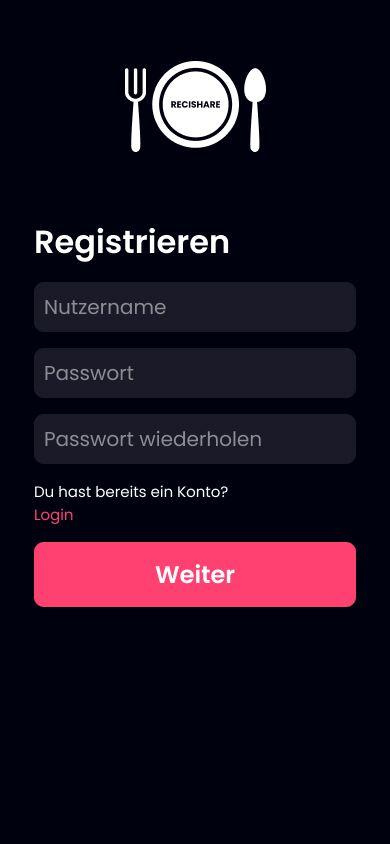
\includegraphics[height=80mm]{images/section7/RegisterView.jpg}
        \label{fig:A71}
        \caption{Registrierenansicht}
    \end{minipage}
    \begin{minipage}
        [t]{0.5\textwidth}
        \centering
        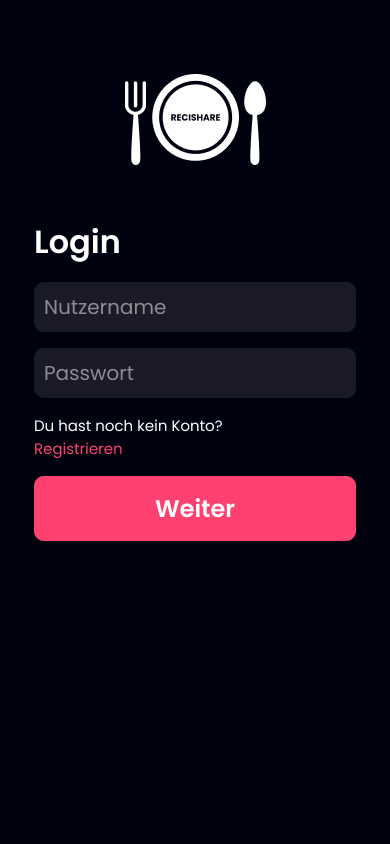
\includegraphics[height=80mm]{images/section7/LoginView.jpg}
        \label{fig:A72}
        \caption{Loginansicht}
    \end{minipage}
\end{figure}

\textbf{Gruppenansicht} $\langle$UI20$\rangle$

Auf der Gruppenansicht (\ref{fig:A73}) kann der Nutzer eine neue Gruppe erstellen, indem er den Namen der neuen Gruppe festlegt und auf "Weiter" drückt. Damit wird die Gruppe in der Datenbank angelegt und der Nutzer tritt dieser bei. Anschließend wird er auf die Hauptansicht $\langle$UI30$\rangle$ weitergeleitet. Alternativ kann der Nutzer auch einer bereits bestehenden Gruppe beitreten. Dazu muss er auf "Gruppe beitreten" drücken, woraufhin sich ein Popup-Fenster öffnet. Hier muss er den Gruppencode eingeben, den jede Gruppe besitzt. Existiert der Gruppencode, so wird der Nutzer der Gruppe hinzugefügt. Auch hier wird der Nutzer auf die Hauptansicht $\langle$UI30$\rangle$ weitergeleitet.

\begin{figure}[!htp]
    \centering
    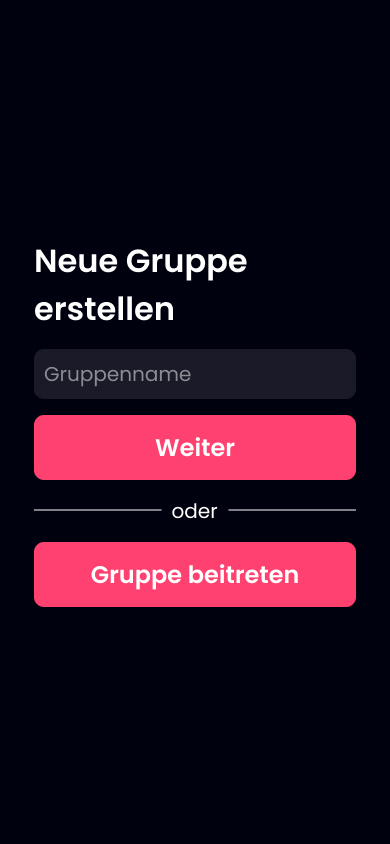
\includegraphics[height=80mm]{images/section7/GroupView.jpg}
    \label{fig:A73}
    \caption{Gruppenansicht}
\end{figure}
\newpage
\textbf{Hauptansicht} $\langle$UI30$\rangle$

In der Hauptansicht (\ref{fig:A74}) kann der Nutzer alle Rezepte aus den Gruppen, in denen er Mitglied ist sehen. Diese kann er nach verschiedenen Faktoren filtern und sortieren. Durch eine Suchleiste kann er außerdem schnell ein gewünschtes Rezept finden. Jedes Rezept wird hier mit Titel, dem ersten Bild, Kochdauer und Schwierigkeitsgrad abgebildet. Durch einen Klick auf das Herzsymbol wird ein Rezept zu den Favoriten hinzugefügt bzw. wieder entfernt. Klickt ein Nutzer auf ein Rezept, so gelangt er zur Rezeptansicht $\langle$UI40$\rangle$. Durch einen Klick auf das Notizblock-Symbol gelangt der Nutzer auf die Rezepterstellenansicht $\langle$UI60$\rangle$.

\begin{figure}[!htp]
    \centering
    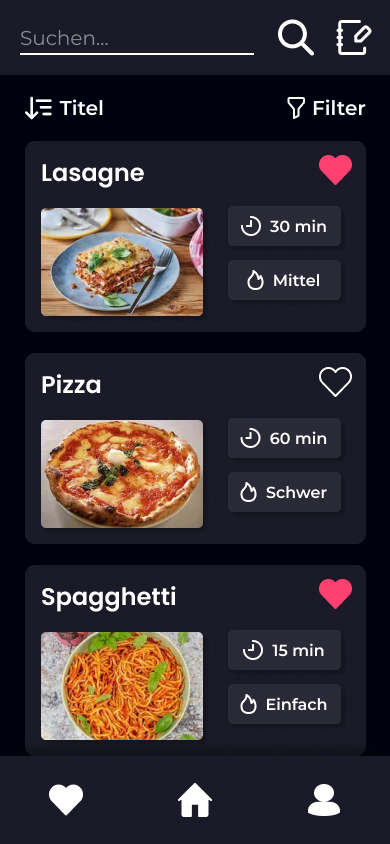
\includegraphics[height=80mm]{images/section7/MainView.jpg}
    \label{fig:A74}
    \caption{Hauptansicht}
\end{figure}

Unten am Bildschirm befindet sich eine Navigationsleiste, die es dem Nutzer ermöglicht, zwischen verschiedenen Ansichten zu wechseln. Durch einen Klick auf das Haus-Symbol gelangt der Nutzer auf die Hauptansicht $\langle$UI30$\rangle$. Durch einen Klick auf das Herz-Symbol gelangt der Nutzer auf die Favoritenansicht $\langle$UI50$\rangle$. Durch einen Klick auf das Personen-Symbol gelangt der Nutzer auf die Verwaltungsansicht $\langle$UI80$\rangle$.

\textbf{Rezeptansicht} $\langle$UI40$\rangle$

In der Rezeptansicht (\ref{fig:A75}) wird ein bestimmtes Rezept angezeigt. Es werden Name, Bilder, Zutaten, Zubereitungsanweisungen, Kochdauer, Schwierigkeitsgrad, Autor und Erstellungsdatum angezeigt. Der Nutzer kann durch anpassen der Portionenzahl automatisch die Zutatenmengen errechnen lassen. Durch einen Klick auf das Herzsymbol wird ein Rezept zu den Favoriten hinzugefügt bzw. wieder entfernt. Ist der Nutzer der Autor des Rezepts, so wird oben ein Stiftsymbol angezeigt. Durch einen Klick auf dieses Symbol gelangt der Nutzer auf die Rezepterstellenansicht $\langle$UI60$\rangle$, die bereits mit dem Rezept befüllt ist. Dort kann er das Rezept bearbeiten. Mit Hilfe des Plus-Symbols über den Bildern kann ein Nutzer außerdem Bilder hochladen, die dann für alle Nutzer im Rezept einsehbar sind. Dies geschieht mit Hilfe des betriebssystemeigenen Dateimanagers. Unten am Bildschirm ist wieder die Navigationsleiste zu finden. Außerdem kann der Nutzer wieder zurück zur vorherigen Ansicht gelangen, indem er auf das Zurück-Symbol oben links klickt.

\begin{figure}[!htp]
    \centering
    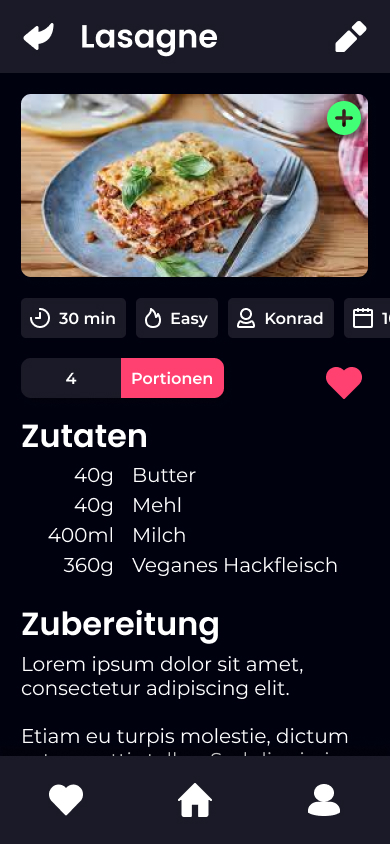
\includegraphics[height=80mm]{images/section7/RecipeView.jpg}
    \label{fig:A75}
    \caption{Rezeptansicht}
\end{figure}

\textbf{Favoritenansicht} $\langle$UI50$\rangle$

Die Favoritenansicht (\ref{fig:A76}) ist identisch zur Hauptansicht $\langle$UI30$\rangle$, nur dass hier nur die favorisierten Rezepte angezeigt werden. Außerdem gibt es hier keinen Button zum Rezepte erstellen.
\newpage
\begin{figure}[!htp]
    \centering
    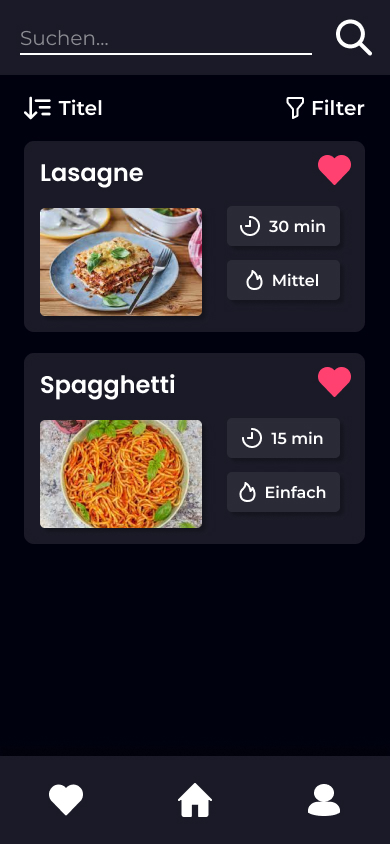
\includegraphics[height=80mm]{images/section7/FavouritesView.jpg}
    \label{fig:A76}
    \caption{Favoritenansicht}
\end{figure}

\textbf{Rezepterstellenansicht} $\langle$UI60$\rangle$

In dieser Ansicht (\ref{fig:A77}) kann ein Nutzer ein neues Rezept erstellen oder bearbeiten. Dazu gibt es verschiedene Eingabefelder, die der Nutzer ausfüllen kann. Diese umfassen den Rezeptnamen, Dauer und Schwierigkeitsgrad sowie die Zubereitungsanweisungen. Außerdem kann er Bilder mit Hilfe des betriebssystemeigenen Dateimanagers hochladen, indem er auf das Bild-Symbol klickt. 
Die Zutaten können mit einem Klick auf das Plus-Symbol hinzugefügt werden. Dazu öffnet sich die Zutatenauswahlansicht, in der der Nutzer die Zutat auswählen kann. Die bereits hinzugefügten Zutaten werden in einer Liste angezeigt und können durch einen Klick auf das Kreuz-Symbol entfernt werden. Ganz unten befindet sich ein Knopf zum Speichern des Rezepts. Durch einen Klick auf das Zurück-Symbol oben links gelangt der Nutzer zurück zur vorherigen Ansicht. Auch hier gibt es wieder die Navigationsleiste.

\begin{figure}[!htp]
    \centering
    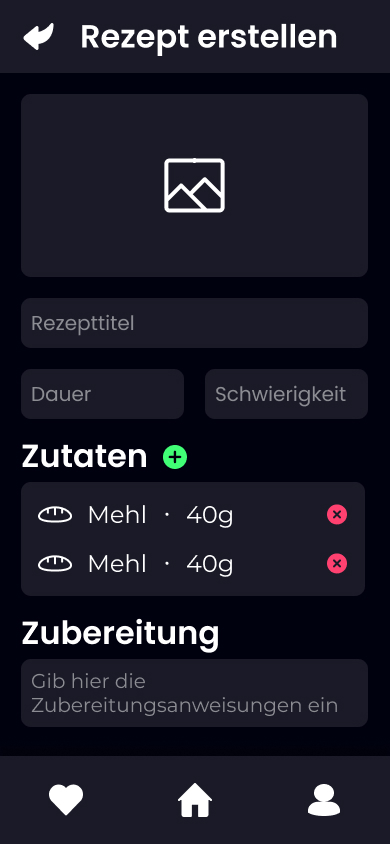
\includegraphics[height=80mm]{images/section7/RecipeCreationView.jpg}
    \label{fig:A77}
    \caption{Rezepterstellenansicht}
\end{figure}

\textbf{Zutatenauswahlansicht} $\langle$UI70$\rangle$

In dieser Ansicht (\ref{fig:A78}) kann der Nutzer Zutaten erstellen. Dazu schreibt er den Namen der Zutat in das Eingabefeld und wählt Einheit und Menge aus. Während der Nutzer die Zutat eingibt sollen automatisch Zutaten gesucht werden, die zum bisher geschriebenen Text passen und als Vorschlag unter dem Eingabefeld angezeigt werden. Durch Klick auf so einen Vorschlag wird der Zutatenname auf diesen Vorschlag gesetzt. Der Nutzer hat außerdem die Möglichkeit ein Icon für die Zutat aus einem Dropdownmenü zu wählen. Durch den "Hinzufügen"-Button wird die Zutat erstellt und der Nutzer gelangt zurück zur Rezepterstellenansicht $\langle$UI60$\rangle$.

\begin{figure}[!htp]
    \centering
    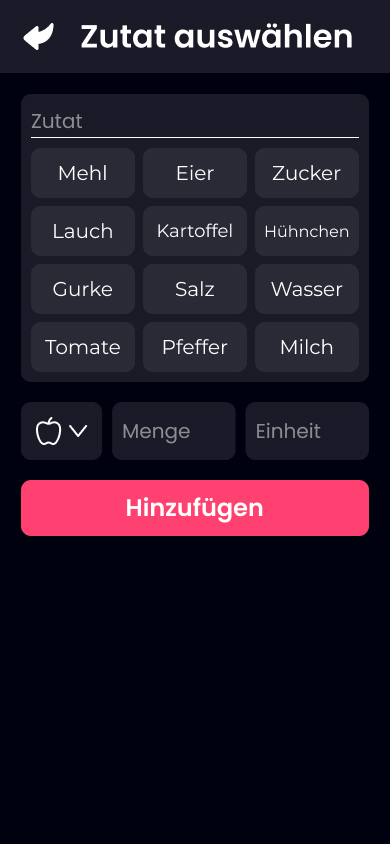
\includegraphics[height=80mm]{images/section7/IngredientPickerView.jpg}
    \label{fig:A78}
    \caption{Rezepterstellenansicht}
\end{figure}

\textbf{Verwaltungsansicht} $\langle$UI80$\rangle$

Die Verwaltungsansicht dient der Verwaltung des Nutzers und seiner Gruppen. Der Nutzer kann seinen Anzeigenamen ändern. Zudem kann er Gruppen austreten, in dem er auf das Kreuz-Symbol neben der entsprechenden Gruppe drückt. Außerdem kann er den Gruppencode mit Hilfe des Teilen-Symbols teilen. Durch das Plus-Symbol gelangt der Nutzer zur Gruppenansicht $\langle$UI90$\rangle$, in der er eine neue Gruppe erstellen kann oder einer bestehenden Gruppe beitritt. Außerdem sieht der Nutzer seine erstellten Rezepte, die er hier mit dem entsprechenden Button entfernen oder bearbeiten kann. Durch Klick auf das Rezept wird man zur entsprechenden Rezeptansicht $\langle$UI40$\rangle$. Mit dem Teilen-Button soll ein Rezept als PDF exportiert werden können.
Zudem kann der Nutzer sich ausloggen mit dem Symbol oben rechts. Daraufhin wird er zur Loginansicht $\langle$UI10$\rangle$weitergeleitet. Auch hier gibt es wieder die Navigationsleiste.

\begin{figure}[!htp]
    \centering
    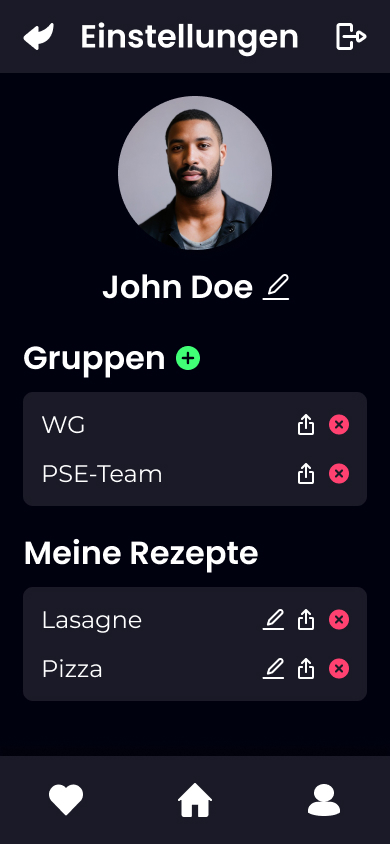
\includegraphics[height=80mm]{images/section7/SettingsView.jpg}
    \label{fig:A79}
    \caption{Verwaltungsansicht}
\end{figure}
\newpage
\section{Technische Produktumgebung}
In diesem Kapitel wird die technische Umgebung des Produktes beschrieben.

\subsection{Software}
\begin{itemize}
    \item Entwicklungsumgebung - Android Studio, IntelliJ
    \item Implementierungssprache der App - Dart
    \item Nuzterverwaltung - Firebase
    \item Client-Betriebssystem - Android 10 oder eine neuere Androidversion
    \item Implementierungssprache des Servers - ?
\end{itemize}

\subsection{Hardware}
\begin{itemize}
    \item Standard Smartphone mit Android Betriebssystem
\end{itemize}

\subsection{Produktschnittstellen}
Die Benutzerschnittstelle wird über ein GUI zur Verfügung gestellt.

\section{Glossar}

\end{document}
